\documentclass{article}
\usepackage{listings}
\usepackage{color}
\usepackage{amsmath}
\usepackage{amsfonts}
\usepackage{amssymb}
\usepackage{caption}
\usepackage{polski}
\usepackage{indentfirst}
\usepackage{graphicx}
\usepackage{pdfpages}
\usepackage{gauss}

\DeclareCaptionType{equ}[][List of equations]
\captionsetup[equ]{labelformat=empty}

%script adding bars in matrix
\usepackage{etoolbox}
\makeatletter
\patchcmd\g@matrix
 {\vbox\bgroup}
 {\vbox\bgroup\normalbaselines}% restore the standard baselineskip
 {}{}
\makeatother

\newcommand{\BAR}{%
  \hspace{-\arraycolsep}%
  \strut\vrule % the `\vrule` is as high and deep as a strut
  \hspace{-\arraycolsep}%
}
\definecolor{dkgreen}{rgb}{0,0.6,0}
\definecolor{gray}{rgb}{0.5,0.5,0.5}
\definecolor{mauve}{rgb}{0.58,0,0.82}

\lstset{frame=tb,
  language=Python,
  aboveskip=3mm,
  belowskip=3mm,
  showstringspaces=false,
  columns=flexible,
  basicstyle={\small\ttfamily},
  numbers=none,
  numberstyle=\tiny\color{gray},
  keywordstyle=\color{blue},
  commentstyle=\color{dkgreen},
  stringstyle=\color{mauve},
  breaklines=true,
  breakatwhitespace=true,
  tabsize=3,
  extendedchars=\true,
  inputencoding=utf8x
}

\lstset{literate={ą}{{\k{a}}}1 {ł}{{\l{}}}1 {ń}{{\'n}}1 {ę}{{\k{e}}}1 {ś}{{\'s}}1 {ż}{{\.z}}1 {ó}{{\'o}}1 {ź}{{\'z}}1 {Ą}{{\k{A}}}1 {Ł}{{\L{}}}1 {Ń}{{\'N}}1 {Ę}{{\k{E}}}1 {Ś}{{\'S}}1 {Ż}{{\.Z}}1 {Ó}{{\'O}}1 {Ź}{{\'Z}}1 }

\begin{document}
\title{Sprawozdanie - Metody numeryczne i optymailzacja}
\author{Jakub Andryszczak 259519,\\ Jakub Żak 244255,\\ Maciej Cierpisz 249163}
\date{}
\maketitle

\newpage
\tableofcontents
%Tutaj zaczyna się wstęp

\newpage
\section{Zadanie nr. 1}
Rozwiązać ręcznie i komputerowo metodą eliminacji Gaussa poniższy układ równań
liniowych. Znaleźć elementy podstawowe (pivots).

\begin{equation}
    \begin{cases}
      2u-v=0 \\
     -u+2v-w=0 \\
     -v+2w-z = 0 \\
     -w+2z=5
    \end{cases}\,.
\end{equation}

Do wykonania tego zadania rozpisano lewą stronę jako macierz 4x4 oraz wektor wynikowy 4x1. Zostały one połączone dzięki czemu otrzymano macierz rozszerzoną 4x5. Poniżej przedstawiono kolejno sposób wyliczania macierzy stosując do tego metodę eliminacji Gaussa.

\[
  \linespread{2}\selectfont
  \addtolength{\arraycolsep}{10pt}
 \begin{gmatrix}[b]
2 & -1 & 0 & 0 & \BAR & 0\\
-1 & 2 & -1 & 0 & \BAR & 0\\
0 & -1 & 2 &-1 & \BAR & 0\\
0 & 0 & -1 & 2 & \BAR & 5
 \rowops
 \add[\cdot \frac1{2}]01
 %\mult{3}{\cdot \left(-\frac2{29}\right)}

 \end{gmatrix}
\]
  Elementem podstawowym dla pierwszej kolumny znajduje się w pierwszej kolumnie i ma wartość 2
\[
  \linespread{2}\selectfont
  \addtolength{\arraycolsep}{10pt}
 \begin{gmatrix}[b]
2 & -1 & 0 & 0 & \BAR & 0\\
0 & \frac3{2} & -1 & 0 & \BAR & 0\\
0 & -1 & 2 &-1 & \BAR & 0\\
0 & 0 & -1 & 2 & \BAR & 5
 \rowops
 \add[\cdot \frac2{3}]12
 %\mult{3}{\cdot \left(-\frac2{29}\right)}

 \end{gmatrix}
\]

\[
  \centering
  \linespread{2}\selectfont
  \addtolength{\arraycolsep}{10pt}
 \begin{gmatrix}[b]
2 & -1 & 0 & 0 & \BAR & 0\\
0 & \frac3{2} & -1 & 0 & \BAR & 0\\
0 & 0 & \frac4{3} &-1 & \BAR & 0\\
0 & 0 & -1 & 2 & \BAR & 5
 \rowops
 \add[\cdot \frac3{4}]23
 %\mult{3}{\cdot \left(-\frac2{29}\right)}

 \end{gmatrix}
\]

\[
  \centering
  \linespread{2}\selectfont
  \addtolength{\arraycolsep}{10pt}
 \begin{gmatrix}[b]
2 & -1 & 0 & 0 & \BAR & 0\\
0 & \frac3{2} & -1 & 0 & \BAR & 0\\
0 & 0 & \frac4{3} &-1 & \BAR & 0\\
0 & 0 & 0 & \frac5{4} & \BAR & 5
 \rowops
 \mult{3}{\cdot \left(-\frac4{5}\right)}
 \add[]23
 \end{gmatrix}
\]
 Kolejnymi elementami podstawowymi są liczby 1.5 , 1.(3) i 1.25
\[
  \centering
  \linespread{2}\selectfont
  \addtolength{\arraycolsep}{10pt}
 \begin{gmatrix}[b]
2 & -1 & 0 & 0 & \BAR & 0\\
0 & \frac3{2} & -1 & 0 & \BAR & 0\\
0 & 0 & \frac4{3} & 0 & \BAR & 4\\
0 & 0 & 0 & 1 & \BAR & 4
 \end{gmatrix}
\]
\[
  \centering
  \linespread{2}\selectfont
  \addtolength{\arraycolsep}{10pt}
 \begin{gmatrix}[b]
2 & -1 & 0 & 0 & \BAR & 0\\
0 & \frac3{2} & 0 & 0 & \BAR & 3\\
0 & 0 & 1 & 0 & \BAR & 3\\
0 & 0 & 0 & 1 & \BAR & 4
 \end{gmatrix}
\]

\[
  \centering
  \linespread{2}\selectfont
  \addtolength{\arraycolsep}{10pt}
 \begin{gmatrix}[b]
2 & 0 & 0 & 0 & \BAR & 2\\
0 & 1 & 0 & 0 & \BAR & 2\\
0 & 0 & 1 & 0 & \BAR & 3\\
0 & 0 & 0 & 1 & \BAR & 4
 \end{gmatrix}
\]

\[
  \centering
  \linespread{2}\selectfont
  \addtolength{\arraycolsep}{10pt}
 \begin{gmatrix}[b]
1 & 0 & 0 & 0 & \BAR & 1\\
0 & 1 & 0 & 0 & \BAR & 2\\
0 & 0 & 1 & 0 & \BAR & 3\\
0 & 0 & 0 & 1 & \BAR & 4
 \end{gmatrix}
\]

Napisano kod w języku Python, który wykonuje eliminację Gaussa bez wyboru elementu podstawowego. Kod znajduje się poniżej.
\begin{center}

\begin{lstlisting}

import numpy as np

def gaussian_elimination(matrix, vector):
    n = len(vector)

    # Tworzenie rozszerzonej macierzy [matrix | vector]
    augmented_matrix = np.hstack((matrix, vector))

    # Eliminacja Gaussa
    for i in range(n):
        # Sprawdzanie, czy na przekątnej jest 0
        if augmented_matrix[i, i] == 0:
            raise ValueError("Zero na przekątnej. Metoda eliminacji Gaussa nie może być kontynuowana.")

        # Eliminacja współczynników pod przekątną
        for j in range(i + 1, n):
            ratio = augmented_matrix[j, i] / augmented_matrix[i, i]
            augmented_matrix[j, i:] = augmented_matrix[j, i:] - ratio * augmented_matrix[i, i:]

    # Rozwiązanie układu równań z wstecznym podstawianiem
    for i in range(n - 1, -1, -1):
        augmented_matrix[i, :] = augmented_matrix[i, :] / augmented_matrix[i, i]
        for j in range(i - 1, -1, -1):
            augmented_matrix[j, :] = augmented_matrix[j, :] - augmented_matrix[j, i] * augmented_matrix[i, :]

    return augmented_matrix

\end{lstlisting}

\end{center}
\section{Zadanie nr. 2}

Rozwiązać poniższy układ równań liniowych metodą eliminacji Gaussa z częściowym
wyborem element podstawowego:

\begin{equation}
  \begin{cases}
    x_{1}+x_{2}+x_{3}=1 \\
   x_{1}+x_{2}+2x_{3}=2 \\
   x_{1} + 2x_{2} +2x_{3}= 1 
  \end{cases}\,.
\end{equation}

Wyjaśnij dlaczego elimin. Gaussa bez wyboru elementu podstawowego nie działa poprawnie.

\[
  \centering
  \linespread{2}\selectfont
  \addtolength{\arraycolsep}{10pt}
 \begin{gmatrix}[b]
1 & 1 & 1 & \BAR & 1\\
1 & 1 & 2 & \BAR & 2\\
1 & 2 & 2 & \BAR & 1
\rowops
\add[-1]02
\add[-1]01
 \end{gmatrix}
\]

\[
  \centering
  \linespread{2}\selectfont
  \addtolength{\arraycolsep}{10pt}
 \begin{gmatrix}[b]
1 & 1 & 1 & \BAR & 1\\
0 & 0 & 1 & \BAR & 1\\
0 & 1 & 1 & \BAR & 0
\rowops
\swap12
 \end{gmatrix}
\]

\[
  \centering
  \linespread{2}\selectfont
  \addtolength{\arraycolsep}{10pt}
 \begin{gmatrix}[b]
1 & 1 & 1 & \BAR & 1\\
0 & 1 & 1 & \BAR & 0\\
0 & 0 & 1 & \BAR & 1
\rowops
\add[-1]21
\add[-1]20
 \end{gmatrix}
\]

\[
  \centering
  \linespread{2}\selectfont
  \addtolength{\arraycolsep}{10pt}
 \begin{gmatrix}[b]
1 & 1 & 0 & \BAR & 0\\
0 & 1 & 0 & \BAR & -1\\
0 & 0 & 1 & \BAR & 1
\rowops
\add[-1]10
 \end{gmatrix}
\]

\[
  \centering
  \linespread{2}\selectfont
  \addtolength{\arraycolsep}{10pt}
 \begin{gmatrix}[b]
1 & 0 & 0 & \BAR & 1\\
0 & 1 & 0 & \BAR & -1\\
0 & 0 & 1 & \BAR & 1
 \end{gmatrix}
\]

Wyjaśnienie dlaczego eliminacja Gaussa bez wyboru elementu podstawowego przedstawiona jest na przykładzie następnego zadania.
Kod różni się w małym stopniu od tego zaimplementowanego w poprzednim zadaniu. Zmiana polega na dodaniu linijek odpowiadających za wybór elementu. Przedstawiona została poniżej.
\begin{center}

  (LINIJKI WYBIERAJĄCE ELEMENT)

  \begin{lstlisting}
    
  \end{lstlisting}
\end{center}
\section{Zadanie nr. 3}

Rozwiązać ręcznie układ równań liniowych:
\begin{equation}
  \begin{cases}
    0,0001x_{1}+x_{2}=1 \\
   x_{1}+x_{2}=2  
  \end{cases}\,.
\end{equation}
przy pomocy eliminacji Gaussa z i bez wyboru elementu podstawowego, zaokrąglając wyniki
obliczeń do trzech znaczących cyfr.

  Początkowo rozwiązano układ nie wybierając elementu podstawowego.

\[
  \centering
  \linespread{2}\selectfont
  \addtolength{\arraycolsep}{10pt}
 \begin{gmatrix}[b]
  -10^{-4} & 1 & \BAR & 1\\
  1 & 1 & \BAR & 2
\rowops
\add[10^4]01
 \end{gmatrix}
\]

\[
  \centering
  \linespread{2}\selectfont
  \addtolength{\arraycolsep}{10pt}
 \begin{gmatrix}[b]
  -10^{-4} & 1 & \BAR & 1\\
  0 & 10^4 & \BAR & 10^4
\rowops
\mult{0}{\cdot \left(-10^4\right)}
\mult{1}{\cdot \left(10^{-4}\right)}
\add[-1]10
 \end{gmatrix}
\]

Podczas sumowania wiersza drugiego zaokrąglono wyniki do trzech liczb znaczących.

\[
  \centering
  \linespread{2}\selectfont
  \addtolength{\arraycolsep}{10pt}
 \begin{gmatrix}[b]
  1 & 0 & \BAR & 0\\
  0 & 1 & \BAR & 1
 \end{gmatrix}
\]

Po przeliczeniu okazało się że wynik jest niepoprawny. Błąd powstaje w drugim równaniu. Podstawiając wartości, które wyszły powstaje równanie:
\begin{equation}
  1=2
\end{equation}
Co jest sprzeczne z prawdą.

W drugim przypadku wybierano element podstawowy co pozwoliło na otrzymanie innego wyniku.

\[
  \centering
  \linespread{2}\selectfont
  \addtolength{\arraycolsep}{10pt}
 \begin{gmatrix}[b]
  -10^{-4} & 1 & \BAR & 1\\
  1 & 1 & \BAR & 2
\rowops
\swap01
 \end{gmatrix}
\]

\[
  \centering
  \linespread{2}\selectfont
  \addtolength{\arraycolsep}{10pt}
 \begin{gmatrix}[b]
  1 & 1 & \BAR & 2\\
  -10^{-4} & 1 & \BAR & 1
 \end{gmatrix}
\]

\[
  \centering
  \linespread{2}\selectfont
  \addtolength{\arraycolsep}{10pt}
 \begin{gmatrix}[b]
  1 & 1 & \BAR & 2\\
  0 & 1 & \BAR & 1
 \end{gmatrix}
\]

\[
  \centering
  \linespread{2}\selectfont
  \addtolength{\arraycolsep}{10pt}
 \begin{gmatrix}[b]
  1 & 0 & \BAR & 1\\
  0 & 1 & \BAR & 1
 \end{gmatrix}
\]
Po podstawieniu wartości, które wyszły okazały się one poprawne dla tego układu równań.
\section{Zadanie nr. 4}
Rozwiązać komputerowo układ równań liniowych:
\begin{equation}
  \begin{cases}
    0,835x_{1}+0,667x_{2}=0,168 \\
   0,333x_{1}+0,266x_{2}=0,067  
  \end{cases}\,.
\end{equation}
Następnie, proszę zmienić (zaburzyć) wartość elementu 2 b z 0.067 na 0.066 i porównać rozwiązanie
z uzyskanym dla układu niezaburzonego. Wyjaśnij dlaczego nastąpiła tak znacząca
zmiana rozwiązania posługując się wskaźnikiem uwarunkowania macierzy systemowej.

  Do wykonania tego zadania wykorzystano algorytm eliminacji Gaussa napisany dla zadania drugiego, podstawiając odpowiednie wartości.
Dla pierwszego przypadku wektor wyjściowy miał wartości:
\begin{equation}
  x =
  \begin{gmatrix}[b]
    1\\
    -1
  \end{gmatrix}
\end{equation}
  W momencie wymiany wartości elementu b wektor wyjściowy prezentuje się następująco:
  \begin{equation}
    x =
    \begin{gmatrix}[b]
      -665,(9)\\
      833,(9)
    \end{gmatrix}
  \end{equation}

Ta dość spora zmiana jest związana ze wskaźnikiem uwarunkowania macierzy, który dla obu przypadków jest dosyć wysoki. Oznacza to, że problem jest źle uwarunkowany. Tego typu zagadnienia nie nadają się do numerycznego rozwiązania, ponieważ już sam błąd wynikający z numerycznej reprezentacji liczb wprowadza nieproporcjonalnie duży błąd w odpowiedzi.
\section{Zadanie nr. 5}
Zaimplementuj dowolny algorytm do faktoryzacji LU i zastosuj do macierzy:
\begin{equation}
  A=
  \begin{gmatrix}[b]
    1 & 2 & 3 & 4\\
    -1 & 1 & 2 & 1\\
    0 & 2 & 1 & 3\\
    0 & 0 & 1 & 1
  \end{gmatrix}
\end{equation}

Wyznacz det(A) na podstawie faktorów. Znajdź rozwiązanie dla układu równań Ax b dla b = $[1...1]^{T}$ , posługując się otrzymanymi faktorami.\\

Zdecydowano się na wykorzystanie algorytm Crout'a. Poniższa implementacja algorytmu na zadanej macierzy polegająca na zastąpieniu macierzy A mnożeniem macierzy dolno i górno trójkątnej o przekątnej składającej się z jedynek. Następnie obliczane są elementy macierzy L i U za pomocą równań bazujących na mnożeniu macierzy L i U oraz przyrownaniu wyników mnożeń do odpowiednich elementów macierzy A. \\
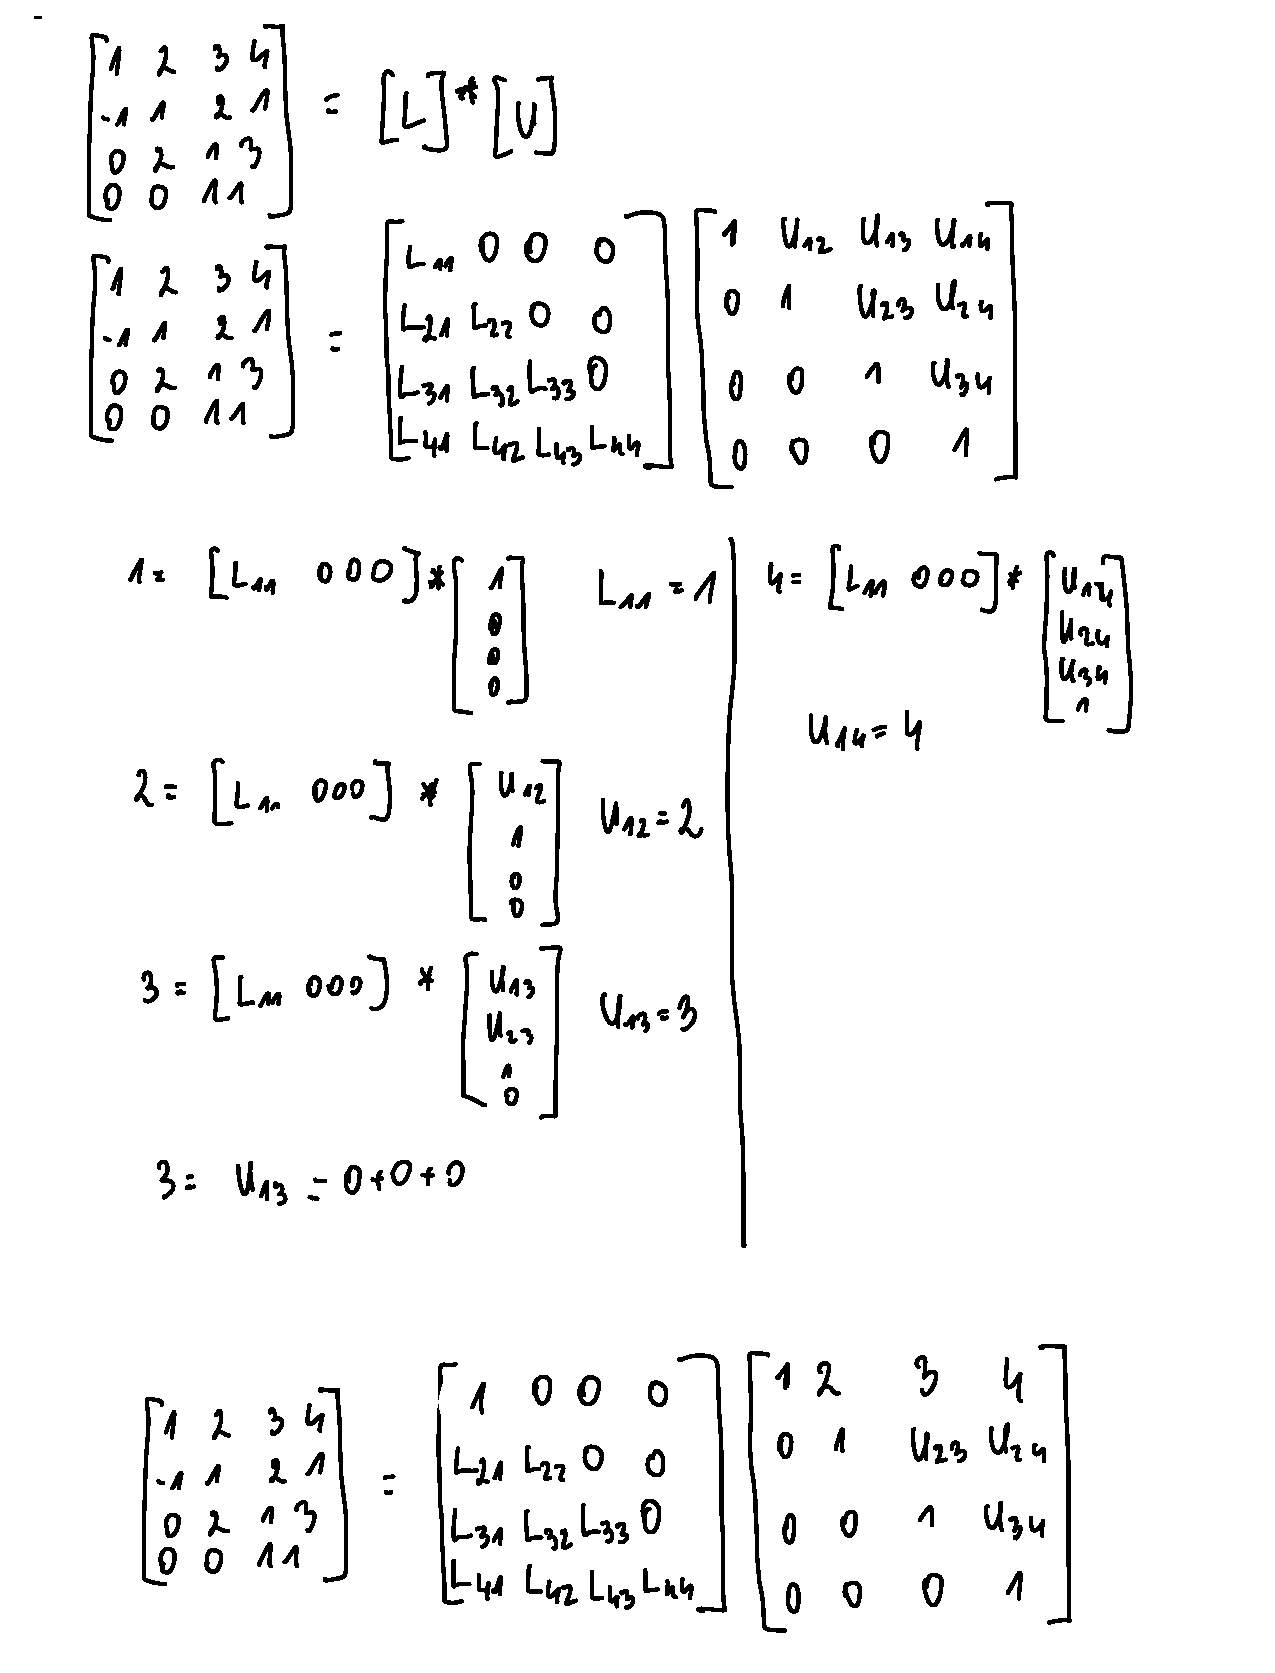
\includepdf[pages=-]{zad5.pdf}

Poniżej implementacja programowa w języku Python:

\begin{lstlisting}
  import numpy as np


def LU(A):
    n = len(A)
    L = np.zeros((n, n))
    U = np.zeros((n, n))

    for i in range(n):
        # Przekątna macierzy L wynosi 1
        L[i][i] = 1

        for j in range(i, n):
            #  Obliczanie elementów macierzy górnej trójkątnej U
            sum = 0
            for k in range(i):
                sum += L[i][k] * U[k][j]
            U[i][j] = A[i][j] - sum

        for j in range(i+1, n):
            #  Oblicznie elementów macierzy dolnej trójkątnej L
            sum = 0
            for k in range(i):
                sum += L[j][k] * U[k][i]
            L[j][i] = (A[j][i] - sum) / U[i][i]

    return L, U

\end{lstlisting}

\section{Zadanie nr. 6}
Przekształć ręcznie poniższą macierz do postaci RREF, wyznacz rank (A) oraz
wskaż kolumny odpowiadające zmiennym podstawowym i wolnym.

\begin{equation}
  A=
  \begin{gmatrix}[b]
  1 & 2 & 2 & 3 & 1\\
  2 & 4 & 4 & 6 & 2\\
  3 & 6 & 6 & 9 & 6\\
  1 & 2 & 4 & 5 & 3 
\end{gmatrix}
\end{equation}

Etapy rozwiązania macierzy przedstawiono poniżej:
\[
  \centering
  \linespread{2}\selectfont
  \addtolength{\arraycolsep}{10pt}
 \begin{gmatrix}[b]
  1 & 2 & 2 & 3 & 1\\
  2 & 4 & 4 & 6 & 2\\
  3 & 6 & 6 & 9 & 6\\
  1 & 2 & 4 & 5 & 3 
 \rowops
 \add[-2]01
 \add[-3]02
 \add[-1]03
\end{gmatrix}
\]
\[
  \centering
  \linespread{2}\selectfont
  \addtolength{\arraycolsep}{10pt}
 \begin{gmatrix}[b]
  1 & 2 & 2 & 3 & 1\\
  0 & 0 & 0 & 0 & 0\\
  0 & 0 & 0 & 0 & 3\\
  0 & 0 & 2 & 2 & 2 
 \rowops
 \swap13
\end{gmatrix}
\]
\[
  \centering
  \linespread{2}\selectfont
  \addtolength{\arraycolsep}{10pt}
 \begin{gmatrix}[b]
  1 & 2 & 2 & 3 & 1\\
  0 & 0 & 2 & 2 & 2\\
  0 & 0 & 0 & 0 & 3\\
  0 & 0 & 0 & 0 & 0
 \rowops
 \mult{1}{\cdot \left(\frac1{2}\right)}
 \mult{2}{\cdot \left(\frac1{3}\right)}
\end{gmatrix}
\]
\[
  \centering
  \linespread{2}\selectfont
  \addtolength{\arraycolsep}{10pt}
 \begin{gmatrix}[b]
  1 & 2 & 2 & 3 & 1\\
  0 & 0 & 1 & 1 & 1\\
  0 & 0 & 0 & 0 & 1\\
  0 & 0 & 0 & 0 & 0
 \rowops
\add[-2]10
\add20
\add[-1]21
\end{gmatrix}
\]
\[
  \centering
  \linespread{2}\selectfont
  \addtolength{\arraycolsep}{10pt}
 \begin{gmatrix}[b]
  1 & 2 & 0 & 1 & 0\\
  0 & 0 & 1 & 1 & 0\\
  0 & 0 & 0 & 0 & 1\\
  0 & 0 & 0 & 0 & 0
\end{gmatrix}
\]

Wartość rank(A) = 3, zmienne podstawowe ($A_{*1},A_{*3},A_{*5}$), zmienne wolne ($A_{*2},A_{*4}$)\\

\section{Zadanie nr. 7}
Zaimplementuj dowolną metodę ortogonalizacji macierzy i wyznacz faktoryzację
QR macierzy:
\begin{equation}
  A=
  \begin{gmatrix}[b]
  -2 & 1 & 2 & 1 \\
  2 & -1 & 2 & 1\\
  2 & 3 & -4 & 5\\
  2 & 3 & 0 & -1 
\end{gmatrix}
\end{equation}

Zaimplementuj dowolną metodę ortogonalizacji macierzy i wyznacz faktoryzację
QR macierzy:
\begin{equation}
  A=
  \begin{gmatrix}[b]
  -2 & 1 & 2 & 1 \\
  2 & -1 & 2 & 1\\
  2 & 3 & -4 & 5\\
  2 & 3 & 0 & -1 
\end{gmatrix}
\end{equation}

Do ortogonalizacji macierzy i stworzenia macierzy Q wykorzytano metodę Grama-Schmidt'a. Początkowo macierz podzielono na 4 osobne wektory wzdłuż kolumn.
Następnie zaczęto wyliczać wartość $u_{1}$. Dla tego przypadku.
\begin{equation}
  u_{1}=a_{1}
\end{equation}
Następnie wyliczono normę dla tego wektora.
\begin{equation}
  ||u_{1}|| = \sqrt{{a_{11}}^2+{a_{12}}^2+{a_{13}}^2+{a_{14}}^2}=4
\end{equation}
Po wyliczeniu wartości $u_{1} oraz ||u_{1}||$ wyliczono pierwszą kolumnę macierzy Q ze wzoru.
\begin{equation}
  q_{1}=\frac{u_{1}}{||u_{1}||} =
  \begin{gmatrix}[b]
    -0.5\\
    0.5\\
    0.5\\
    0.5
  \end{gmatrix}
\end{equation}

Kolejne kolumny zostały przeliczane stosując wzoru jak w poprzednim przykładzie. Następnie zsumowano je tworząc macierz Q 4x4.
\begin{equation}
  Q =
  \begin{gmatrix}[b]
    -0.5 & 0.5 & 0.5 & 0.5\\
    0.5 & -0.5 & 0.5 & 0.5\\
    0.5 & 0.5 & -0.5 & 0.5\\
    0.5 & 0.5 & 0.5 & -0.5
  \end{gmatrix}
\end{equation}
W przypadku wyliczenia macierzy R możemy ją wyliczyć przekształcając wzór
\begin{equation}
  A = QR / * {Q}^T
\end{equation}
\begin{equation}
  AQ^{T} = QR{Q}^T
\end{equation}
Z własności macierzy ortogonalnych wynika następująca zależność
\begin{equation}
  Q^{T}Q = I
\end{equation}
I jest macierzą jednostkową, która jest neutralna dla mnożenia macierzy co za tym idzie nasz wzór wygląda następująco
\begin{equation}
  A{Q}^T = R
\end{equation}
Podstawiając do tego wzoru wartości otrzymujemy że
\begin{equation}
  R =
  \begin{gmatrix}[b]
    -0.5 & 0.5 & 0.5 & 0.5\\
    0.5 & -0.5 & 0.5 & 0.5\\
    0.5 & 0.5 & -0.5 & 0.5\\
    0.5 & 0.5 & 0.5 & -0.5
  \end{gmatrix}
  *
  \begin{gmatrix}[b]
    -2 & 1 & 2 & 1 \\
  2 & -1 & 2 & 1\\
  2 & 3 & -4 & 5\\
  2 & 3 & 0 & -1
  \end{gmatrix}
\end{equation}
\begin{equation}
  R =
  \begin{gmatrix}[b]
    4 & 2 & -2 & 2\\
    0 & 4 & -2 & 2\\
    0 & 0 &  4 & -2\\
    0 & 0 & 0 & 4
  \end{gmatrix}
\end{equation}

Stworzono kod w Python'ie, który wykonuje wyżej wytłumaczoną Faktoryzację QR.\\

\begin{lstlisting}
  import numpy as np

def gram_schmidt(A):
    m, n = A.shape
    Q = np.zeros((m, n))
    R = np.zeros((n, n))

    for i in range(n):
        #  Obliczenie ortogonalnego wektora q_i
        q = A[:, i]
        for j in range(i):
            # Odejmowanie rzutu q na każde q_j
            R[j, i] = np.dot(Q[:, j], A[:, i])
            q = q - R[j, i] * Q[:, j]
        # Obliczenie wielkości q (która jest przekątną R)
        R[i, i] = np.linalg.norm(q)
        # Unikanie dzielenia przez zero
        if R[i, i] == 0:
            raise ValueError("Matrix A has linearly dependent vectors")
        # Step 3: Normalize q to get the orthonormal vector q_i
        Q[:, i] = q / R[i, i]
    return Q, R

\end{lstlisting}
\newpage
\section{Zadanie nr. 8}

Niech Ax = b , gdzie , symbol  oznacza iloczyn Kroneckera,
 jest macierzą jednostkową,  C jest macierzą losową wygenerowaną z rozkładu
równomiernego (rand), M = 200, N = 30, oraz   (rozkład normalny - randn).
Rozwiąż układ równań różnymi metodami bezpośrednimi (eliminacja Gaussa, faktoryzacja LU,
faktoryzacja QR) i porównaj metody ze względu na czas wykonywania się algorytmów i błąd
aproksymacji rozwiązania.\\

Badaniu poddano własne implementacje algorytmów oraz metody dostępne w bibliotece scipy.
Poniej zestawiono wyniki badań w postaci zmierzonych czasów wykonania poszczegolnych algorytmów oraz obliczone błędy aproksymacji.
\begin{figure}[h]
  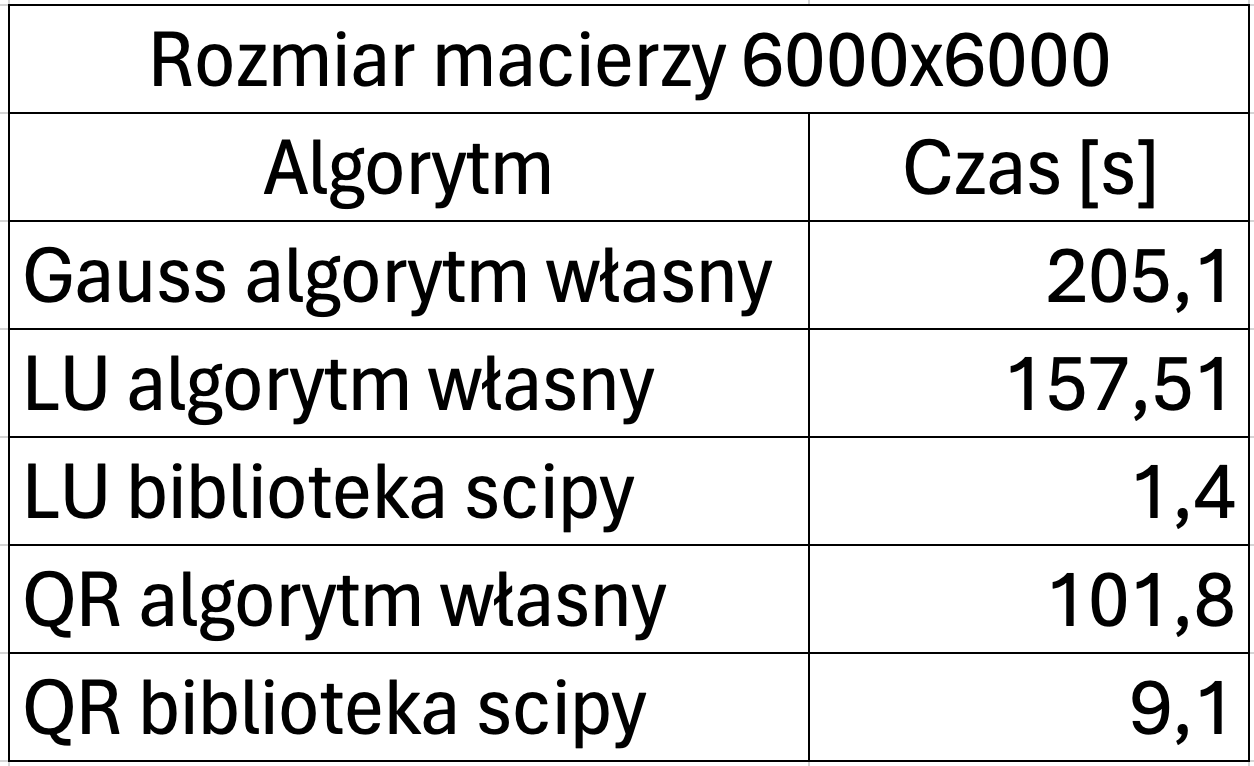
\includegraphics[scale=0.3]{image.png}
  \centering
  \captionsetup[Tabela]{name=New Table Name}
  \caption*{Tabela. 1 Wykaz czasów wykonania algorytmów}
  \end{figure}

  \begin{figure}[h]
    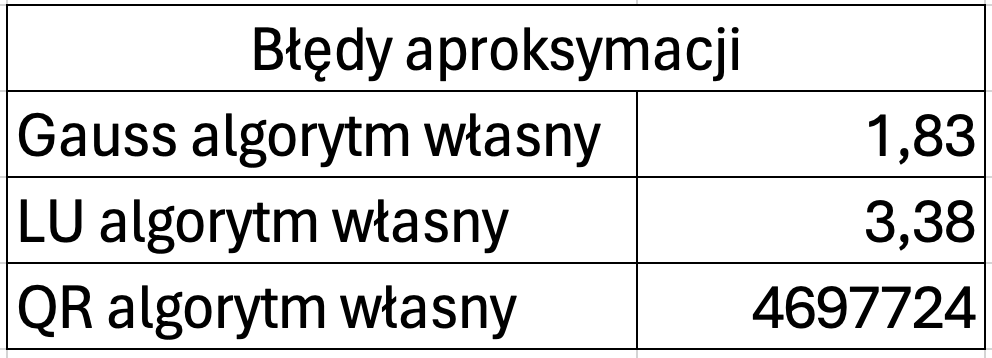
\includegraphics[scale=0.4]{image2.png}
    \centering
    \caption*{Tabela. 2 Wykaz błędów aproksymacji algorytmów}
    \end{figure}
    
    \newpage
\section{Zadanie nr. 9}
Znajdź prądy gałęziowe zakładając, że wszystkie rezystancje wynoszą 20 Ohm.

\begin{equ}[!ht]
\caption{Równania napięciowe}
\begin{equation}
  \begin{cases}
    2I_{3}-2I_{4}=1\\
    -I_{3}-I_{5}=1\\
    2I_{6}-2I_{5}=1 
  \end{cases}\,.
\end{equation}
\end{equ}

\begin{equ}[!ht]
  \caption{Równania prądowe}
  \begin{equation}
    \begin{cases}
      I_{2}+I_{3}-I_5=0\\
      I_{5}+I_{6}-I_1=0\\
      I_{4}-I_{2}-I_6=0\\
      I_1-I_3-I_4=0
    \end{cases}\,.
  \end{equation}
  \end{equ}

  \begin{equ}[!ht]
    \caption{Równania prądowe}
    \begin{equation}
      \begin{cases}
        I_1 - I_3 - I_4 = 0\\
        I_2 + I_3-I_5 = 0\\
        -I_3 - I_5 = 1\\
        2I_3 - 2I_4 = 1\\
        -2I_5 + 2I_6 = 1\\
        -I_2 + I_4 -I_6 = 0
      \end{cases}\,.
    \end{equation}
    \end{equ}
    \newpage
    Kod obliczający wartości szukanych prądów
    \begin{lstlisting}
      import numpy as np
      from numpy.linalg import solve
      
      #Inicjalizacja macierzy A i wektora b
      A = np.array([ [1, 0, -1, -1, 0, 0],
                    [0, 1, 1, 0, -1, 0],
                    [0, 0, -1, 0, -1, 0],
                    [0, 0, 2, -2, 0, 0],
                    [0, 0, 0, 0, -2, 2],
                    [0, -1, 0, 1, 0, -1],])
      
      b = np.array([0, 0, -1, -1, -1, 0],dtype=float)
      
      #Obliczenie wyników metodą eliminacji Gaussa z pivotingiem
      x = solve(A,b)
    \end{lstlisting}

    \begin{equ}[!ht]
      \caption{Wyniki obliczeń}
      \begin{equation}
        \begin{cases}
          I_{1}=1\\
          I_{2}=0.5\\
          I_{3}=0.25\\
          I_{4}=0.75\\
          I_{5}=0.75\\
          I_{6}=0.25
        \end{cases}\,.
      \end{equation}
      \end{equ}



\section{Wnioski}
Laboratoria miały za zadanie przedstawienie metod rozwiązywania macierzy takich jak: Eliminacja Gaussa, Faktoryzacja LU i QR.
Po przeprowadzeniu wcześniej określonych zadań 
Eliminacja Gaussa jest prostą metodą przekształcania macierzy i najdokładniejsza w porównaniu do pozostałych dwóch, natomiast porównując czas wykonania szczególnie dla macierzy o dużych rozmiarach pracuje najwolniej.
Faktoryzacja LU polega na przedstawieniu macierzy w postaci wyniku mnożenia macierzy dolnotrójkątnej L z macierzą górnotrójkątną U. Jest ona szybsza w porównaniu do eliminacji Gaussa, ale posiada większy błąd aproksymacji.
W przypadku faktoryzacji QR polega ona na wyznaczeniu macierzy ortogonalnej do niej Q, a następnie przekształcając wzór $ A = QR $ Wyliczamy macierz R. Jest to najszybszy sposób przekształcania, aczkolwiek posiada on największy błąd. \end{document} 